% Template LaTeX file for DAFx-19 papers
%
% To generate the correct references using BibTeX, run
%     latex, bibtex, latex, latex
% modified...
% - from DAFx-00 to DAFx-02 by Florian Keiler, 2002-07-08
% - from DAFx-02 to DAFx-03 by Gianpaolo Evangelista
% - from DAFx-05 to DAFx-06 by Vincent Verfaille, 2006-02-05
% - from DAFx-06 to DAFx-07 by Vincent Verfaille, 2007-01-05
%                          and Sylvain Marchand, 2007-01-31
% - from DAFx-07 to DAFx-08 by Henri Penttinen, 2007-12-12
%                          and Jyri Pakarinen 2008-01-28
% - from DAFx-08 to DAFx-09 by Giorgio Prandi, Fabio Antonacci 2008-10-03
% - from DAFx-09 to DAFx-10 by Hannes Pomberger 2010-02-01
% - from DAFx-10 to DAFx-12 by Jez Wells 2011
% - from DAFx-12 to DAFx-14 by Sascha Disch 2013
% - from DAFx-15 to DAFx-16 by Pavel Rajmic 2015
% - from DAFx-16 to DAFx-17 by Brian Hamilton 2016
% - from DAFx-18 to DAFx-19 by Dave Moffat 2019
%
% Template with hyper-references (links) active after conversion to pdf
% (with the distiller) or if compiled with pdflatex.
%
% 20060205: added package 'hypcap' to correct hyperlinks to figures and tables
%                      use of \papertitle and \paperauthorA, etc for same title in PDF and Metadata
% 05/02/2019: Package 'hypcap' removed, and replaced with 'caption', to allow for the inclusion
%			of a CC UP licence.
%
% 1) Please compile using latex or pdflatex.
% 2) If using pdflatex, you need your figures in a file format other than eps! e.g. png or jpg is working
% 3) Please use "paperftitle" and "pdfauthor" definitions below

%------------------------------------------------------------------------------------------
%  !  !  !  !  !  !  !  !  !  !  !  ! user defined variables  !  !  !  !  !  !  !  !  !  !  !  !  !  !
% Please use these commands to define title and author(s) of the paper:
\def\papertitle{Real-Time Implementation of the Elasto-Plastic Bow Model applied to Finite-Difference Schemes}
\def\paperauthorA{Silvin Willemsen}
\def\paperauthorB{Stefania Serafin}
\def\paperauthorC{Stefan Bilbao}

% Authors' affiliations have to be set below

%------------------------------------------------------------------------------------------
\documentclass[twoside,a4paper]{article}
\usepackage{dafx_19}
\usepackage{amsmath,amssymb,amsfonts,amsthm}
\usepackage{euscript}
\usepackage[latin1]{inputenc}
\usepackage[T1]{fontenc}
\usepackage{ifpdf}

\usepackage[english]{babel}
\usepackage{caption}
\usepackage{subfig} % or can use subcaption package
\usepackage{color}
\newenvironment{rcases}
  {\left.\begin{alignedat}{2}}
  {\end{alignedat}\right\rbrace}
\DeclareMathOperator{\sgn}{sgn}
\setcounter{page}{1}
\ninept

\usepackage{times}
% Saves a lot of ouptut space in PDF... after conversion with the distiller
% Delete if you cannot get PS fonts working on your system.

% pdf-tex settings: detect automatically if run by latex or pdflatex
\newif\ifpdf
\ifx\pdfoutput\relax
\else
   \ifcase\pdfoutput
      \pdffalse
   \else
      \pdftrue
\fi

\ifpdf % compiling with pdflatex
  \usepackage[pdftex,
    pdftitle={\papertitle},
    pdfauthor={\paperauthorA, \paperauthorB},
    colorlinks=false, % links are activated as colror boxes instead of color text
    bookmarksnumbered, % use section numbers with bookmarks
    pdfstartview=XYZ % start with zoom=100% instead of full screen; especially useful if working with a big screen :-)
  ]{hyperref}
  \pdfcompresslevel=9
  \usepackage[pdftex]{graphicx}
%  \usepackage[figure,table,hypcap=true]{caption}
\else % compiling with latex
  \usepackage[dvips]{epsfig,graphicx}
  \usepackage[dvips,
    colorlinks=false, % no color links
    bookmarksnumbered, % use section numbers with bookmarks
    pdfstartview=XYZ % start with zoom=100% instead of full screen
  ]{hyperref}
  % hyperrefs are active in the pdf file after conversion
%  \usepackage[figure,table,hypcap=true]{caption}
\fi
  \usepackage[hypcap=true]{caption}
\title{\papertitle}

%-------------SINGLE-AUTHOR HEADER STARTS (uncomment below if your paper has a single author)-----------------------
%\affiliation{
%\paperauthorA \,\sthanks{This work was supported by the XYZ Foundation}}
%{\href{http://dafx2019.bcu.ac.uk/}{Digital Media Technology Lab} \\ Birmingham City University \\ Birmingham, UK \\ {\tt \href{mailto:dafx2019@gmail.com}{dafx2019@gmail.com}}}
%-----------------------------------SINGLE-AUTHOR HEADER ENDS------------------------------------------------------

%---------------TWO-AUTHOR HEADER STARTS (uncomment below if your paper has two authors)-----------------------
\twoaffiliations{
\paperauthorA, \paperauthorB}
{{Multisensory Experience Lab, CREATE,} \\ Aalborg University Copenhagen\\
  Copenhagen, Denmark\\ {\tt \href{mailto:sil@create.aau.dk}{\{sil, sts\}@create.aau.dk}}}
{\paperauthorC}
{ Acoustics and Audio Group \\ University of Edinburgh\\
    Edinburgh, UK\\
     {\tt \href{mailto:s.bilbao@ed.ac.uk}{s.bilbao@ed.ac.uk}}}
%-------------------------------------TWO-AUTHOR HEADER ENDS------------------------------------------------------

%---------------THREE-AUTHOR HEADER STARTS (uncomment below if your paper has three authors)-----------------------
% \threeaffiliations{
% \paperauthorA \,\sthanks{This work was supported by the XYZ Foundation}}
% {\href{http://dafx2019.bcu.ac.uk/}{Digital Media Technology Lab} \\ Birmingham City University \\ Birmingham, UK \\ {\tt \href{mailto:dafx2019@gmail.com}{dafx2019@gmail.com}}}
% {\paperauthorB \,\sthanks{Thanks to the predecessors for the templates}}
% {\href{http://dafx2018.web.ua.pt/}{IEETA} \\ University of Aveiro \\ Aveiro, Portugal \\ {\tt \href{mailto:dafx2018_papers@ua.pt}{dafx2018\_papers@ua.pt}}}
% {\paperauthorC \,\sthanks{Illustrious contributor}}
% {\href{http://www.acoustics.ed.ac.uk}{Acoustics and Audio Group,} \\ University of Edinburgh\\ Edinburgh, UK\\ {\tt \href{mailto:dafx17@ed.ac.uk}{dafx17@ed.ac.uk}}}
%-------------------------------------THREE-AUTHOR HEADER ENDS------------------------------------------------------

%----------------FOUR-AUTHOR HEADER STARTS (uncomment below if your paper has four authors)-----------------------
% \fouraffiliations{
% \paperauthorA \,\sthanks{This work was supported by the XYZ Foundation}}
% {\href{http://dafx2019.bcu.ac.uk/}{Digital Media Technology Lab} \\ Birmingham City University \\ Birmingham, UK \\ {\tt \href{mailto:dafx2019@gmail.com}{dafx2019@gmail.com}}}
% {\paperauthorB \,\sthanks{Thanks to the predecessors for the templates}}
% {\href{http://dafx2018.web.ua.pt/}{IEETA} \\ University of Aveiro \\ Aveiro, Portugal \\ {\tt \href{mailto:dafx2018_papers@ua.pt}{dafx2018\_papers@ua.pt}}}
% {\paperauthorC \,\sthanks{Illustrious contributor}}
% {\href{http://www.acoustics.ed.ac.uk}{Acoustics and Audio Group,} \\ University of Edinburgh\\ Edinburgh, UK\\ {\tt \href{mailto:dafx17@ed.ac.uk}{dafx17@ed.ac.uk}}}
% {\paperauthorD \,\sthanks{This guy is a very good fellow}}
% {\href{http://dafx16.vutbr.cz}{SPLab} \\ Brno University of Technology \\ Brno, Czech Republic \\ {\tt \href{mailto:dafx16@vutbr.cz}{dafx16@vutbr.cz}}}
%-------------------------------------FOUR-AUTHOR HEADER ENDS------------------------------------------------------

\begin{document}
% more pdf-tex settings:
\ifpdf % used graphic file format for pdflatex
  \DeclareGraphicsExtensions{.png,.jpg,.pdf, .eps} 
\else  % used graphic file format for latex
  \DeclareGraphicsExtensions{.eps}
\fi

\maketitle

\begin{abstract}
This is the template file for the proceedings of the 22\textsuperscript{nd} International Conference on Digital Audio Effects (DAFx-19).
This template has been derived from WASPAA'99 templates and aims at producing conference proceedings in electronic form.
The format is essentially the one used for ICASSP conferences.
Please use either this \LaTeX{} or the accompanying Word formats when preparing your submission.
The templates are available in electronic form on \href{http://dafx2019.bcu.ac.uk/}{http://dafx2019.bcu.ac.uk/}.
\end{abstract}

\section{Introduction}
\label{sec:intro}
Bow models:

The elasto-plastic 
\section{Stiff String}
Using the subscripts $t$ and $x$ to denote a single derivative with respect to time and space respectively, the partial differential equation of the damped stiff string is defined as \cite{Bilbao2009}
\begin{equation}\label{eq:PDE}
    u_{tt} = c^2u_{xx}-\kappa^2u_{xxxx}-2\sigma_0u_t+2\sigma_1u_{txx},
\end{equation}
where $c = \sqrt{T/\rho A}$ is the wave speed (in m/s) with tension $T$ (in N), material density $\rho$ (in kg$\cdot$m$^{-3}$) and cross-sectional area $A$ (in m$^2$), $\kappa = \sqrt{EI/\rho A}$ is the stiffness coefficient (in m$^2$/s) with Young's Modulus $E$ (in Pa) and area moment of inertia $I$ (in m$^4$) and frequency independent and frequency dependent damping coefficients $\sigma_0 \geq 0$ and $\sigma_1 \geq 0$.
\section{Elasto-Plastic Bow Model}
As opposed to less complex bow models, such as the hyperbolic [source] and exponential [source] models, the elasto-plastic bow model assumes that the friction between the bow and the string is caused by a large quantity of bristles, each of which contributes to the total amount of friction. The bristles are assumed to be stiff springs with damping and can 'break' after a given break-away displacement. An extra term can be added to \eqref{eq:PDE} to include the bowing interaction
\begin{equation}
    \begin{aligned}
    \label{eq:bowingTerm}
        u_{tt} = \hdots - \delta(x-x_\text{B})f(v, z),
    \end{aligned}
\end{equation}
with spatial Dirac delta function $\delta(x-x_\text{B})$ applying the bowing function $f$ at bowing position $x_\text{B}$. The bowing function is dependent on the relative velocity between the string at the bowing point and the bow
\begin{equation}\label{eq:relVel}
  v = u_t(x_\text{B}) - v_\text{B}
\end{equation}
and the aforementioned average bristle displacement $z$. The bowing function is defined as
\begin{equation}\label{eq:forceFunction}
    f(v, z) = s_0z + s_1\dot z + s_2v
\end{equation}
where $s_0$ is the bristle stiffness (in N/m), $s_1$ is the damping coefficient and $s_2$ 

Moreover, the rate of change of $z$ is
\begin{equation}\label{eq:zdot}
    \dot z(v, z) = v\bigg[1-\alpha(v, z)\frac{z}{z_\text{ss}(v)}\bigg]
\end{equation}
where $z_\text{ss}$ is the steady-state function
\begin{equation}
    z_\text{ss} = \frac{\sgn(v)}{s_0}\Big[f_\text{c}+(f_\text{s}-f_\text{c})e^{-(v/v_\text{s})^2}\Big].
\end{equation}
with stribeck velocity $v_\text{s}$ (in m/s), coulomb force $f_\text{c} = f_\text{N}\mu_\text{c}$ and stiction force $f_\text{s} = f_\text{N}\mu_\text{s}$ (both in N). Here $f_\text{N}$ is the normal force (in N) and $\mu_\text{c}$ and $\mu_\text{s}$ are the dynamic and static friction coefficient respectively. 
Furthermore, the adhesion map between the bow and the string is defined as
\begin{equation}\label{eq:adhesionMap}
\alpha(v, z) 
    \begin{cases}
    \begin{rcases}
        &0 & |z| < z_\text{ba}\\
       &\alpha_\text{m}(v,z)&\ \, z_\text{ba}<|z|<z_\text{ss}(v)\\        &1 &|z|>z_\text{ss}(v)
        \end{rcases}\text{if}\  \sgn(v)=\sgn(z)\\
        0\hspace{107pt}\text{if}\  \sgn(v)\neq\sgn(z),
    \end{cases}
\end{equation}
where the transition between the elastic and plastic behaviour is defined as
\begin{equation}
    \alpha_\text{m} = \frac{1}{2}\bigg[1+\sin\bigg(\pi\frac{z-\frac{1}{2}(z_\text{ss}(v)+z_\text{ba})}{z_\text{ss}(v)-z_\text{ba}}\bigg)\bigg],
\end{equation}
with break-away displacement $z_\text{ba}$, i.e. where the bristles start to break, as mentioned at the beginning of this section. A visualisation of the adhesion map can be found in Figure \ref{fig:alphaPlot}.

\textbf{In order to get the symmetry seen Figure \ref{fig:alphaPlot}, these need to be the equations:}

\begin{equation}\label{eq:adhesionMap}
\alpha(v, z) 
    \begin{cases}
    \begin{rcases}
        &0 & |z| < z_\text{ba}\\
       &\alpha_\text{m}(v,z)&\ \, z_\text{ba}<|z|<|z_\text{ss}(v)|\\        &1 &|z|>|z_\text{ss}(v)|
        \end{rcases}\text{if}\  \sgn(v)=\sgn(z)\\
        0\hspace{107pt}\text{if}\  \sgn(v)\neq\sgn(z),
    \end{cases}
\end{equation}

\begin{equation}
    \alpha_\text{m} = \frac{1}{2}\bigg[1+\sgn(z)\sin\bigg(\pi\frac{z-\sgn(z)\frac{1}{2}(|z_\text{ss}(v)|+z_\text{ba})}{|z_\text{ss}(v)|-z_\text{ba}}\bigg)\bigg],
\end{equation}

\begin{figure}[ht]
\centerline{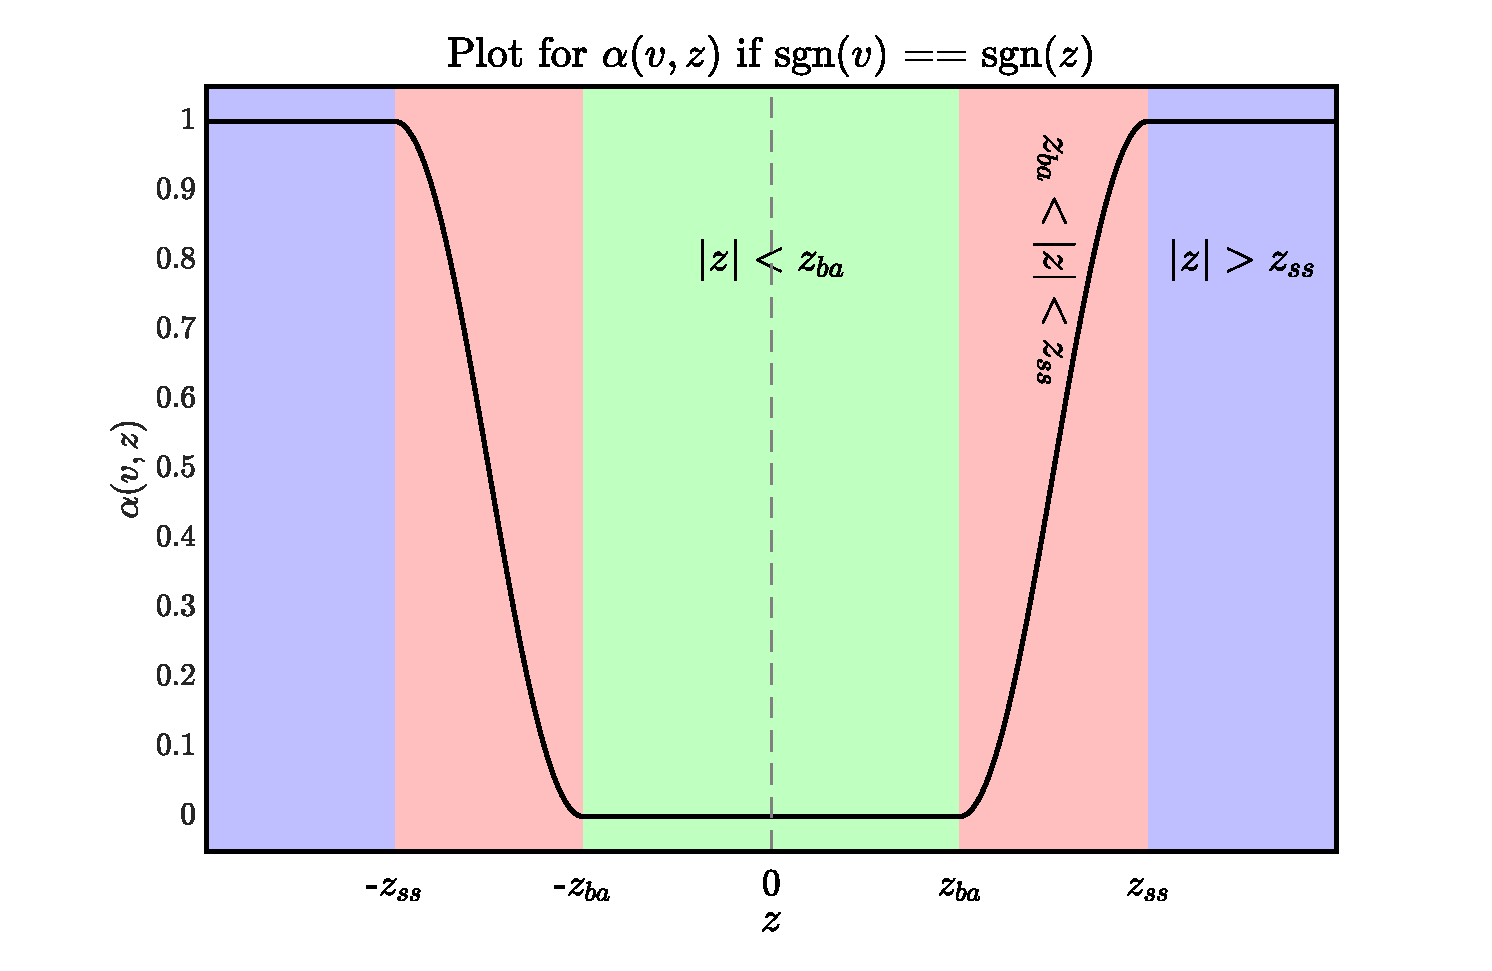
\includegraphics[width=1.0\columnwidth]{alphaPlot.eps}}
\caption{\label{fig:alphaPlot}{\it A plot of the adhesion map $\alpha(v,z)$ plotted against $z$ when the signs of $v$ and $z$ are the same. The different regions of the map are shown with the coloured areas.}}
\end{figure}

\section{Discretisation}\label{sec:discretisation}
Equation \eqref{eq:PDE} can be discretised at times $t = nk$, with sample $n \in \mathbb{N}$ and time-step $k = 1 / f_\text{s}$ with sample-rate $f_\text{s}$ and locations $x = lh$, with grid points $l \in [0,N]$, where $N + 1$ is the total number of grid points and grid spacing $h$ which needs to abide the following condition 
\begin{equation}
    h \geq h_\text{min} = \sqrt{\frac{c^2k^2+4 \sigma_1k+\sqrt{(c^2k^2+4\sigma_1k)^2+16\kappa^2k^2}}{2}}.
\end{equation}
The closer $h$ is to $h_\text{min}$, the more accurate the scheme will be. 
Approximations for the derivatives in the equations found in \ref{eq:PDE} are described in the following way: 
\begin{subequations}\label{eq:approximations}
    \begin{align}
        % \label{eq:secondSpacey}\delta_{yy}u_l^n &= \frac{1}{h^2}\big(u_{m+1}^n - 2u_m^n + u_{m-1}^n\big),\\
        %  \label{eq:fourthSpace}\delta_xxxx &= \frac{1}{h^4}\big(u_{l+2}^n - 4u_{l+1}^2 + 6 u_{l}^n - 4u_{l-1}^n + u_{l-2}^n\big),\\
        \label{eq:centerTime}
        u_{t} &\approx \delta_{t\cdot} u^n_l = \frac{1}{2k}\big(u_l^{n+1}-u_l^{n-1}\big),\\
        \label{eq:secondTime}
        u_{tt} &\approx \delta_{tt}u_l^n = \frac{1}{k^2} \big(u_l^{n+1} - 2u_l^n + u_l^{n-1}\big),\\
        \label{eq:secondSpacex}
        u_{xx} &\approx \delta_{xx}u_l^n = \frac{1}{h^2}\big(u_{l+1}^n - 2u_l^n + u_{l-1}^n\big),\\
        u_{txx} &\approx 
        \begin{aligned}[t]\delta_{t-}\delta_{xx}u_l^n =& \; \frac{1}{hk^2}\big(u_{l+1}^n - 2u_l^2 + u_{l-1}^n \\
        &- u_{l+1}^{n-1} + 2u_l^{n-1} - u_{l-1}^{n-1}\big),
        \end{aligned}\\
        \label{eq:fourthSpacex}
        u_{xxxx} &\approx\begin{aligned}[t] \delta_{xxxx}u_l^n = \frac{1}{h^4}\big(&u_{l+2}^n - 4u_{l+1}^n + 6u_l^n \\
        &- 4u_{l-1}^n +u_{l-2}^n\big),
        \end{aligned}
    \end{align}
\end{subequations}
Using the discretised variable $u_l^n$ is $u(x,t)$ at the $n$th time step and the $l$th point on the string, and the approximations shown in \eqref{eq:approximations} we can discretise \eqref{eq:bowingTerm}
\begin{equation}
  \begin{aligned}
    \label{eq:FDS}
        \delta_{tt} u_l^n = &\: c^2 \delta_{xx} u_l^n -\kappa^2\delta_{xxxx} u_l^n - 2\sigma_0\delta_{t\cdot} u_l^n
        \\ 
        &+ 2\sigma_1\delta_{t-}\delta_{xx}u_l^n - J(x_\text{B}^n)f(v, z).
    \end{aligned}
\end{equation}
where
and the discrete relative velocity is
\begin{equation}\label{eq:discRelVel}
v = I(x_\text{B}^n)\delta_{t\cdot}u_l^n -  v_\text{B}.
\end{equation}
where $I(x_\text{B}^n)$ and $J(x_\text{B}^n)$ are an interpolator and a spreading function around time-variant bowing point $x_\text{B}^n$ (see Appendix \ref{app:interpol}).
At the bowing point we need to iteratively solve for two unknown variables: the relative velocity between the bow and the string $v$ and the mean bristle displacement $z$ of the bow.
We can solve \eqref{eq:FDS} at $x_\text{B}^n$ using \eqref{eq:discRelVel} and identity
\begin{equation}
    \delta_{tt}u_l^n = \frac{2}{k}\big(\delta_{t\cdot}u_l^n-\delta_{t-}u_l^n\big),
\end{equation}
resulting in 
\begin{equation}
\label{eq:stiffStringFDS}
\begin{aligned}
\frac{2}{k}v &+ \frac{2}{k}v_\text{B} - I(x_\text{B}^n) \delta_{t-}u_l^n = \; c^2 I(x_\text{B}^n)\delta_{xx} u_l^n \\
&-\kappa^2I(x_\text{B}^n)\delta_{xxxx} u_l^n - 2\sigma_0v
- 2\sigma_0v_\text{B}\\
&+ 2\sigma_1I(x_\text{B}^n)\delta_{t-}\delta_{xx}u_l^n - J(x_\text{B}^n)f(v, z).
\end{aligned}
\end{equation}
Recalling \eqref{eq:forceFunction}, this can be rewritten to
\begin{align}\label{eq:newtonFunction}
    &s_0z+s_1\dot z+(s_2 + \frac{2}{k} + 2\sigma_0)v + b = 0 \quad \text{where} \\
    & \begin{aligned}b =& \: \frac{2}{k}v_\text{B}-\frac{2}{k}\delta_{t-}u_l^n - c^2 \delta_{xx} u_l^n +\kappa^2\delta_{xxxx} u_l^n \\
    &+ 2\sigma_0v_\text{B}
- 2\sigma_1\delta_{t-}\delta_{xx}u_l^n,
\end{aligned}
\end{align}
where $b$ can be pre-computed as its terms are not dependent on $v$ or $z$.
Newton's method (or Newton-Raphson) is defined as
\begin{equation}
    x^{i+1} = x^{i} - \frac{g(x^i)}{g'(x^i)} \quad \text{while} \quad |x^{i+1}-x^i| > \epsilon
\end{equation}
where $g(x)$ is an arbitrary function dependent on to-be-calculated variable $x$ at iteration index $i$. The calculation is done until the difference between the unknown variable at the next iteration and the current iteration is smaller than a threshold $\epsilon$.

As we need to find the roots of \eqref{eq:zdot}, $g$ with $x=\dot z$ is defined as
\begin{equation}
   g(\dot z) = v\bigg[1-\alpha(v, z)\frac{z}{z_\text{ss}(v)}\bigg] -  \dot z(v,z) = 0,
\end{equation}
and
\begin{equation}
    \dot z^{i+1} = \dot z^i - \frac{g(\dot z^i)}{g'(\dot z^i)}
\end{equation}
where
\begin{equation}
    g'(\dot z^i) = -\frac{s_1}{h(s_2+\frac{2}{k} + 2\sigma_0)}\frac{dg(\dot z^i)}{dv} + \frac{k}{2}\frac{dg(\dot z^i)}{dz} - 1.
\end{equation}
In the iteration, we use the newly calculated value for $\dot z$ and the values of $z$ and $\dot z$ at the previous time step to calculate an estimate of $z$ using the trapezoidal rule
\begin{equation}
    z^n = z^{n-1} + \frac{k}{2}(\dot z^{i+1} + \dot z^{n-1}).
\end{equation}
Inserting this into \eqref{eq:newtonFunction} we can caluclate $v$ using
\begin{equation}
    v = \frac{-s_0z-s_1\dot z-b}{s_2 + \frac{2}{k} + 2\sigma_0}.
\end{equation}

\section{Conclusions}
This template can be found on the conference website.
For changing the number of author affiliations (1 to 4), uncomment the corresponding regions in the template \texttt{tex} file.
Please, submit full-length papers (max.~8 pages both oral and poster presentations).
Submission is fully electronic and automated through the Conference Web Submission System.
DO NOT send us papers directly by e-mail.

\section{Acknowledgments}
Many thanks to the great number of anonymous reviewers!

%\newpage
\nocite{*}
\bibliographystyle{IEEEbib}
\bibliography{DAFx19_tmpl} % requires file DAFx19_tmpl.bib

\section{Appendix: Interpolation and Spreading Operators}
\label{app:interpol}
In this section, the interpolator and spreading operator introduced in Section \ref{sec:discretisation} will be explained.

The simplest way to select a grid point $l_\text{B}$ from bowing position $x_\text{B}$ on a discrete string is $l_\text{B} = \text{floor}(x_\text{B}/h)$. Applied to a gridfunction $u_l$ yields
\begin{equation}
    I_0(x_\text{B})u_l = u_{l_\text{B}}.
\end{equation}
More accurate would be to use linear interpolation 
\begin{equation}\label{eq:linearInterpolation}
     I_1(x_\text{B})u_l =
      (1-\alpha_\text{B})u_{l_\text{B}}+ \alpha_\text{B}u_{l_\text{B}+1}
\end{equation}
where $\alpha_\text{B} = x_\text{B}/h - l_\text{B}$ is the fractional remainder of the flooring operation. Even more accurate would be to use cubic interpolation:
% \begin{equation}\label{eq:cubicInterpolation}
% \begin{aligned}
%      I_3(x_\text{B})u_{l_\text{B}} =&  \frac{\alpha_\text{B}(\alpha_\text{B}-1)(\alpha_\text{B} - 2)}{-6}u_{l_\text{B}-1}+\\
%      &\frac{(\alpha_\text{B}-1)(\alpha_\text{B}+1)(\alpha_\text{B}-2)}{2}u_{l_\text{B}}+  \frac{\alpha_\text{B}(\alpha_\text{B}+1)(\alpha_\text{B} - 2)}{-2}u_{l_\text{B}+1} \\
%      &+ \frac{\alpha_\text{B}(\alpha_\text{B}+1)(\alpha_\text{B} - 1)}{6}u_{l_\text{B}+2}
%      \end{aligned}
% \end{equation}
\begin{equation}
I_3(x_\text{B}) =
     \begin{cases}
    \hfil 0, & l < l_{\text{B}} - 1\\
    \hfil \alpha_\text{B}(\alpha_\text{B}-1)(\alpha_\text{B} - 2)/{-6}, & l = l_{\text{B}} - 1\\
    \hfil (\alpha_\text{B}-1)(\alpha_\text{B}+1)(\alpha_\text{B}-2)/2, & l = l_{\text{B}}\\
    \hfil \alpha_\text{B}(\alpha_\text{B}+1)(\alpha_\text{B} - 2)/{-2}, & l = l_{\text{B}} + 1\\
    \hfil \alpha_\text{B}(\alpha_\text{B}+1)(\alpha_\text{B} - 1)/6, & l = l_{\text{B}} +2,\\
    \hfil 0, & l > l_\text{B} + 2
    \end{cases}
    \end{equation}
spreading operator $J$ can be defined as linear \cite{Bilbao2009}:
\begin{equation}\label{eq:linearInterpolation}
     J_1(x_\text{B}) = \frac{1}{h}
     \begin{cases}
    \hfil 0, & l < l_{\text{B}}\\
    \hfil (1-\alpha_\text{B}), & l = l_{\text{B}}\\
    \hfil \alpha_\text{B}, & l = l_{\text{B}} + 1\\
    \hfil 0, & l > l_\text{B} + 1
\end{cases}
\end{equation}
or cubic:
\begin{equation}\label{eq:cubicInterpolation}
     J_3(x_\text{B}) = \frac{1}{h}
     \begin{cases}
    \hfil 0, & l < l_{\text{B}} - 1\\
    \hfil \alpha_\text{B}(\alpha_\text{B}-1)(\alpha_\text{B} - 2)/{-6}, & l = l_{\text{B}} - 1\\
    \hfil (\alpha_\text{B}-1)(\alpha_\text{B}+1)(\alpha_\text{B}-2)/2, & l = l_{\text{B}}\\
    \hfil \alpha_\text{B}(\alpha_\text{B}+1)(\alpha_\text{B} - 2)/{-2}, & l = l_{\text{B}} + 1\\
    \hfil \alpha_\text{B}(\alpha_\text{B}+1)(\alpha_\text{B} - 1)/6, & l = l_{\text{B}} +2,\\
    \hfil 0, & l > l_\text{B} + 2
\end{cases}
\end{equation}
\end{document}
